%!BIB program = bibtex
\documentclass[9pt, twocolumn, twoside, lineno]{pnas-new}
% Use the lineno option to display guide line numbers if required.

% PNAS研究论文模板
\templatetype{pnasresearcharticle} % Choose template 
% {pnasresearcharticle} = Template for a two-column research article
% {pnasmathematics} %= Template for a one-column mathematics article
% {pnasinvited} %= Template for a PNAS invited submission
% \usepackage{cite}
	
% 文章标题:“流域尺度的水资源利用体系:过渡框架和发展困局”
\title{Water resource utilization regimes at a basin scale: transition framework and development traps}

% Use letters for affiliations, numbers to show equal authorship (if applicable) and to indicate the corresponding author
% 作者列表
\author[a, b]{Shuang Song}  % 宋爽,一作
\author[a, b, 1]{Shuai Wang}  % 王老师,通讯
\author[a, b]{Bojie Fu}  % 傅老师
\author[c, d]{Xutong Wu}  % 武旭同

% 机构列表
\affil[a]{ % 北师大地表国重
	State Key Laboratory of Earth Surface Processes and Resource Ecology, 
	Faculty of Geographical Science, 
	Beijing Normal University, 
	Beijing 100875, 
	P.R. China
}
\affil[b]{ % 北师大地理学部
	Institute of Land Surface System and Sustainability, 
	Faculty of Geographical Science, 
	Beijing Normal University, 
	Beijing 100875, 
	P.R. China
}
\affil[c]{ % 北大城环
	College of Urban and Environmental Sciences, 
	Peking University, 
	Beijing 100871, 
	P.R. China
}
\affil[d]{ % 中科院生态中心
	State Key Laboratory of Urban and Regional Ecology, 
	Research Center for Eco-Environmental Sciences, 
	Chinese Academy of Sciences, 
	Beijing 100085, 
	P.R. China 
}

% Please give the surname of the lead author for the running footer
% 领衔作者
\leadauthor{Song} 

% Please add a significance statement to explain the relevance of your work
% PNAS特有的“Significance陈述”,用不超过120个字来说明研究的意义和亮点
\significancestatement{
	% Authors must submit a 120-word maximum statement about the significance of their research paper written at a level understandable to an undergraduate educated scientist outside their field of speciality. The primary goal of the significance statement is to explain the relevance of the work in broad context to a broad readership. The significance statement appears in the paper itself and is required for all research papers.
	Water, a key resource to support the sustainable development of human societies, whose natural cycle has been modified by growing socio-economic processes. We propose a new method with an integrated indicator to detect water utilization regimes and applying them on the Yellow River Basin, a typical overexploited basin in China. After sketching changes of relationships between development and water utilization within the Yellow River Basin, we summarized a general transition framework. By predicting widespread development traps, it can be a useful guideline for basins all around the world in their sustainable developing trajectories. 
}

% Please include corresponding author, author contribution and author declaration information
\authorcontributions{ % 作者的相应贡献
	Shuai Wang and Bojie Fu designed this research,
	Shuang Song performed the research and analysed data,
	Shuang Song, Xutong Wu wrote the paper.
}
\authordeclaration{ % 利益冲突陈述
	The authors declare no competing interests.
}

% 如果有共同一作的情况,则uncomment下面这行代码的注释
%\equalauthors{\textsuperscript{1}A.O.(Author One) contributed equally to this work with A.T. (Author Two) (remove if not applicable).}

% 通讯作者信息
\correspondingauthor{\textsuperscript{1}To whom correspondence should be addressed. E-mail: shuaiwang@bnu.edu.cn}

% 关键词,三到五个
% At least three keywords are required at submission. Please provide three to five keywords, separated by the pipe symbol.
\keywords{Regime shifts $|$ Human-water relationship $|$ Water resource management $|$ Water utilization $|$ Sustainable development} 

%tag 摘要
\begin{abstract}
	In the context of regime shifts, understanding the complex relationship between human societies and water resources utilization provides underlying supports to development in a coordinated way at a basin scale. However, there is still lacking of effective method to detect regime shifts of water utilization, with much fewer attempts to develop theoretical models to explain their transition phases as well. Here, by integrating three different dimensions of water utilization (stress, tendentiousness and pattern), we develop an Integrated Water Resources Utilization (IWRU) Index at a basin scale to detect regime shifts. By applying this index to the Yellow River Basin, China, we summarized a general transition framework of regimes, which gives a sketch of relationships between human societies and their water utilization. Based on the framework, transition phases within the three regimes and accompanying development traps can be well understood, as a useful guideline for the Yellow River to develop in a coordinated way.
\end{abstract}


\dates{This manuscript was compiled on \today}
\doi{\url{www.pnas.org/cgi/doi/10.1073/pnas.XXXXXXXXXX}}


\begin{document}

\maketitle
\thispagestyle{firststyle}
\ifthenelse{\boolean{shortarticle}}{\ifthenelse{\boolean{singlecolumn}}{\abscontentformatted}{\abscontent}}{}
% If your first paragraph (i.e. with the \dropcap) contains a list environment (quote, quotation, theorem, definition, enumerate, itemize...), the line after the list may have some extra indentation. If this is the case, add \parshape=0 to the end of the list environment.

% tag 引言第一段
% 水资源在人类世的重要性,是支持人类社会发展的基础。
\dropcap{W}ater, at “the centre of the planetary drama of the Anthropocene”, is not only essential for myriad Earth system processes, but also supporting development of human societies in various aspects \cite{gleesonIlluminatingWaterCycle2020}. 
% 但同时, 人类的改造也深刻影响了自然水循环过程, 相关变化可能影响人水系统功能的不利转变,并带来发展困局。
At the same time, however, human's modification has profoundly influenced the water cycle which may lead adverse changes to functions of human-water systems, resulting in various development traps \cite{cummingLinkingEconomicGrowth2018}. 
% 大河流域常是经济和文明发展的中心,同时也是面临人类世压力挑战的主要地区,亟需综合水资源治理以实现可持续发展。
Facing major challenges in the Anthropocene, many of the world's big river basins, also hot spots of economy and civilization, are urgently in need for integrated water resources management toward sustainability \cite{bestAnthropogenicStressesWorld2019}. 
% 因此理解人类社会发展与水资源利用的复杂关系,对此有帮助。
Therefore, understanding the complex relationship between human societies and water resources utilization, and its evolution provides underlying supports to development in a coordinated way, at a basin scale.

% tag 引言第二段
% Regime 和 Regime shift 的定义。
Regime is a stable state of system’s structure and function, whose large and persistent changes may lead to substantive impacts on the outcomes of system with widespread cascading effects, defined as regime shifts \cite{rochaCascadingRegimeShifts2018a}.
% 人水系统中的水资源功能
Within human-water systems, water have several key functions, the most important of which is supplying for human societies in sustainable development based on a complex structure of water utilization. 
% 水资源利用 regime shift
However, inter-connected human interference, involving water withdrawal, dam constructions and water managements have significantly changed water functions and induced regime shifts in water utilization
\cite{falkenmarkUnderstandingWaterResilience2019}.
% 稳态转换随着社会发展增加
These regime shifts, triggered by gradual or abrupt drivers, are likely to occur more often as societies' development increasing their pressure or stuck in traps at a basin scale.
% Regime 过渡性的存在
As a result, many large river basins had gone through water utilization regimes of accelerated exploitation, over-exploitation, and integrated governance, as such it is a reasonable assumption that there is a transition pattern within regime shifts. 
% 过渡性有助于理解流域存在的问题
Sketching the transition of water utilization regimes, therefore, can help to understand and predict development traps, which is crucial for integrated management and coordinated development towards sustainability at a basin scale.
% 对过渡性的研究还很少
Despite pervasive and important, there is still lacking of effective method to define the water utilization regimes and detect regime shifts, with much fewer attempts to develop theoretical models to explain their transition phases as well. 


% Tag 引言第三段
% 前人已经从不同维度刻画了人水关系.
Development of societies by using water resources has been going on for at least thousands of years. Although its regime shifts and transition phases are not fully understood yet, water utilization has been depicted and studied from different dimensions.
% 首先,因为水资源的稀缺性和全球用水量的增加,受到最广泛关注的是人类社会面临的水资源压力。
Firstly, since water resources are scarce, the most widespread concern is the rising stresses on human societies to use water resources.
Even though the stocks of water in artificial reservoirs are helpful to water resources availability, greater water utilization stresses had become a major constraint to development, because of significant increment in water withdrawals and larger shares of inflexible water utilization during the last century.
\cite{postelHumanAppropriationRenewable1996, greveGlobalAssessmentWater2018a, qinFlexibilityIntensityGlobal2019}
% 其次,随着工业迅猛发展和生态建设的需要,社会对水资源的利用的倾向性也发生了转变。
Secondly, as the need of industrial and ecological developments, tendentiousness of water utilization changed with. 
Despite a major water utilization of agricultural irrigation dominating most river basins, there are noticeable growths and preferential tendentiousness in the economy profits and water consumption regarding industry or services, leading potential conflicts between different sectors.
\cite{liuWaterScarcityAssessments2017, florkeWaterCompetitionCities2018}
% 最后,由于水的可用性本质上是区域问题,水资源利用的格局也很重要
Thirdly, since water distribution and utilization are inherently basinal concerns, patterns of also play an important role.
% 全球总的取水量很少,但缺水地区很多
Although only 10\% of available water is withdrawn on global average, about 30\% of population live in highly water-stressed areas,
where dominated sectors of water utilization are various as well. 
\cite{wadaWedgeApproachWater2014, okiGlobalHydrologicalCycles2006}
% 此外,人类活动还在改变这一格局
In addition, human activities are still changing this pattern, since positive impacts caused by human interventions mostly occur in upper regions whereas aggravated water resources downstream, in many basins around the world.
\cite{veldkampWaterScarcityHotspots2017}
% 将三种视角结合,就是“水资源利用体系”。
Although existing researches have evaluated the aspects of water resource utilization from these different dimensions, we still cannot obtain a coherent understanding of regime shifts regard to social development and water utilization, without integrating them.


% tag 引言最后一段
% 这里我们整合了三个方向,提出了描绘流域人水关系的指数
Here, by integrating three above mentioned dimensions of water utilization, we develop an Integrated Water Resources Utilization (IWRU) Index at a basin scale to give a sketch of relationships between human societies and their water utilization.
% 使用案例研究
Then, by applying this index to the Yellow River Basin, China, we analysed water utilization regimes and their shifts in this typical basin of anthropogenic impacts, with change points detection and contribution decomposition methods following.
% 指出发展困局
In addition, combining data analysis, we identify causes of the regime shifts. 
% 最后总结出一般性框架
Finally, refer to the existing theories, we summarized a general transition framework of water utilization regimes, which can be a useful guideline for basins to predict development traps and to develop in a coordinated way.


\section*{Results}
\subsection*{Detection of Water utilization regimes}
% 这一节主要展示IWRU的变化趋势和WUR的划分
With two significant points detected, the trend of IWRU index are split into three periods, whose slopes are various and mainly contributed by different dimensions (stress, tendentiousness or pattern of water utilization, see Methods) (Figure~\ref{fig:IWRU}).
\begin{figure}%[htbp]
	\centering
	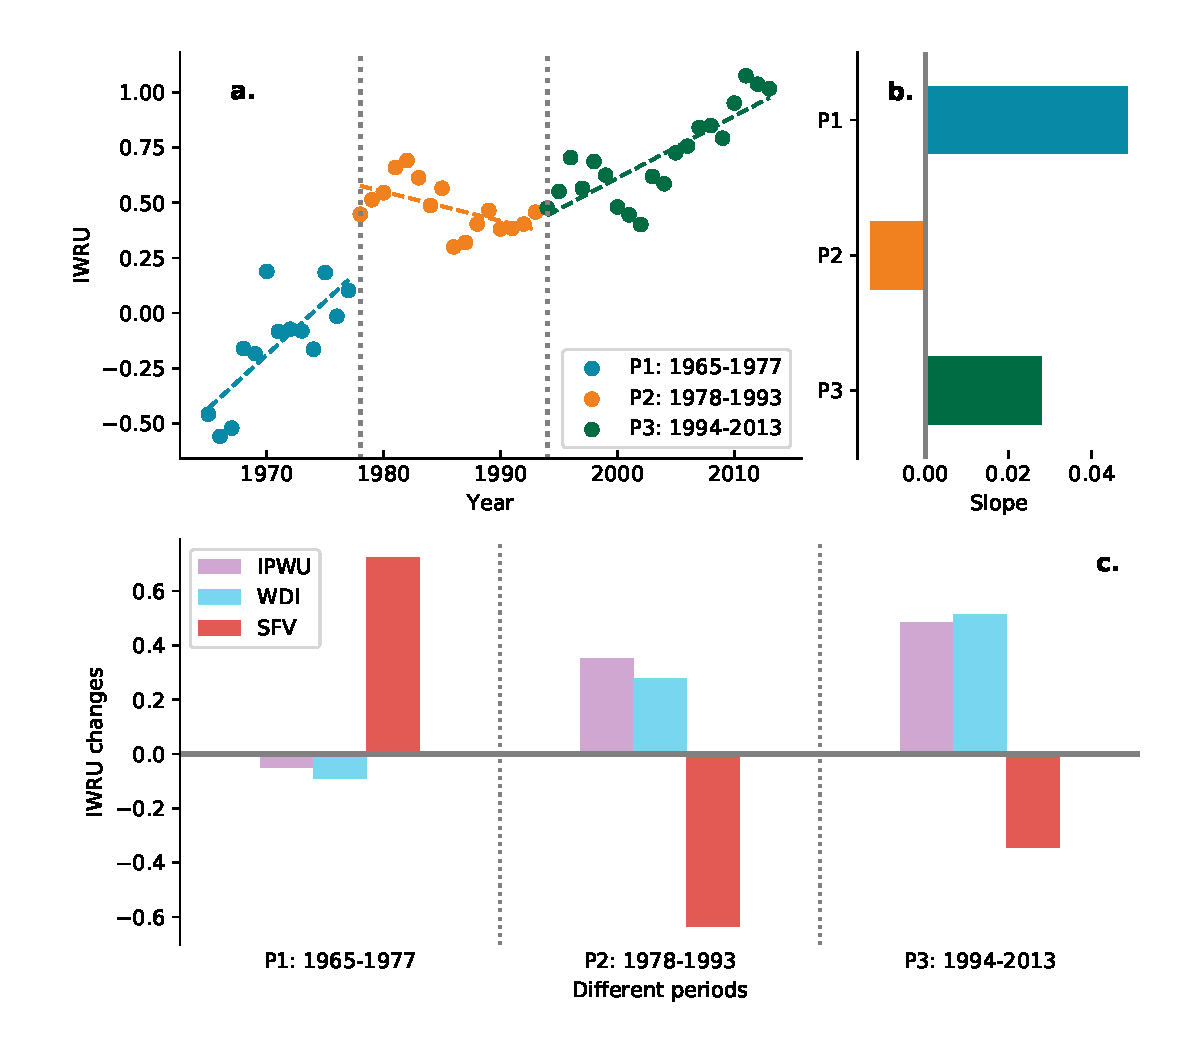
\includegraphics[width=\linewidth]{../../figures/main_text/index.pdf}
	\caption{Changes of the IWRU index. 
	\textbf{A,} with two change points in 1978 and 1994, three periods were detected in trend of the IWRU.
	\textbf{B,} changes of IWRU in three periods have various slopes, while the second period have a negative growths rate.
	\textbf{C,} changes of the IWRU within three certain periods, which have different main contributors.
	}
	\label{fig:IWRU}
\end{figure}
% 接下来分句介绍每个阶段的特征
% 第一阶段
In the first period (P1, 1965-1978), the IWRU index had a rapidly increasing and the lightening of water stresses made the most striking contribution (+0.722), while tendentiousness and pattern of the water utilization had slight negative contribution (-0.048 and -0.09 respectively).
% 第二阶段
In the second period (P2, 1979-1994), the IWRU index experienced a slight drop, despite positive contributions of tendentiousness and pattern of water utilization (+0.352 and +0.279 respectively), because of increasing stresses on water resource playing a larger negative role (-0.636). 
% 第三阶段
However, as the further increasing of positive contributions of water utilization tendentiousness (+0.485) and pattern (+0.515), and decelerations of water stresses (-0.344, 46\% less than P2) in the third period (P3, 1995-2013), a positive growth of the IWRU returned.
% 总而言之,每个阶段都由水资源利用的不同维度提供最大的正向作用
As a result, each period has a different most striking positive contributor to IWRU: P1 is stress; P2 is tendentiousness; and P3 is pattern.

% 用水三个维度的组合呈现出阶段特征明显
Combining these three dimensions' net contribution to IWRU further, ratios of the contributions of the three dimensions clustered clearly by different time periods, indicating three regimes (Figure~\ref{fig:phases}).
\begin{figure}%[htbp]
	\centering
	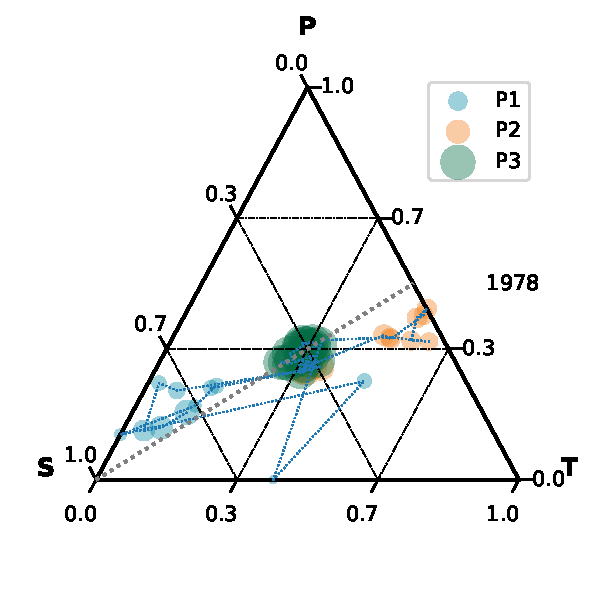
\includegraphics[width=\linewidth]{../../figures/main_text/phases.pdf}
	\caption{Combination of three dimensions (S: stresses; T: tendentiousness; P: pattern) in different periods. 
	Size of the points denoting average of absolute value of each indicator: the mean of the P1 phase is 0.10, while 0.14, 0.19 in P2 and P3.
	The red indicator line in this ternary plot denotes 1:1 contributions between tendentiousness (T) and patterns (P).
	Two key change points (1978, 1994), along with the beginning (1965) and the ending (2013) of research period, are labelled.}
	\label{fig:phases}
\end{figure}
% 第一阶段到第二阶段
At the very beginning (1965) and throughout the whole P1, water utilization regime dominated by high stress. After then, it experienced a shift to low stress since 1978, with a change in the proportion of contributions between tendentiousness and pattern, too.
% 第三阶段集中
Finally, the three dimensions' contribution were much similar in P3, making the points highly concentrated at the centre of the ternary diagram for that period.


%tag 结果2
\subsection*{Differences between water utilization regimes}
% 在不同的维度下各阶段进行对比,可以发现不同的水资源利用体系间存在明显差异。
The differences between the water utilization regimes are reflected in changes of all three dimensions.
\begin{figure*}%[htbp]
	\centering
	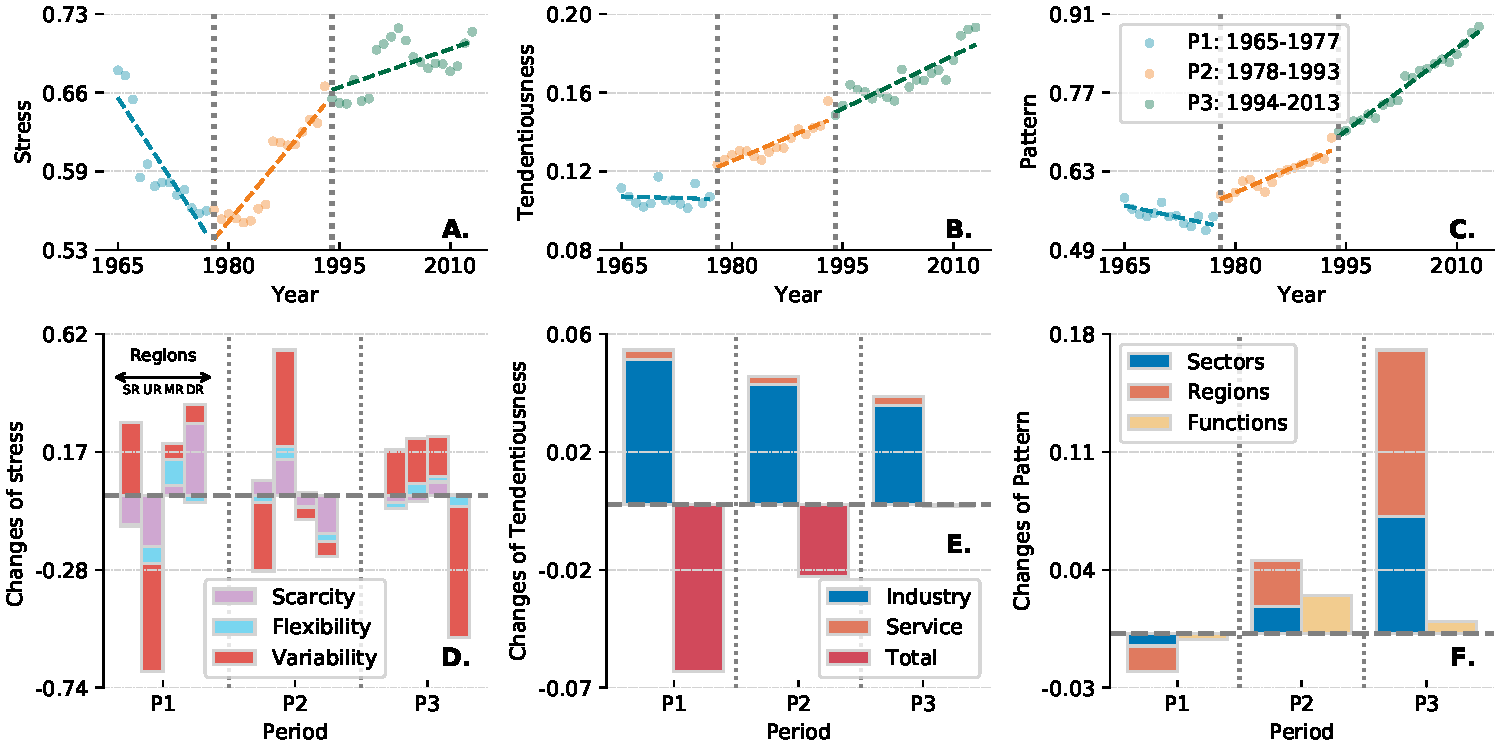
\includegraphics[width=\linewidth]{../../figures/main_text/dimensions.pdf}
	\caption{
		Changes in different dimensions of water resources utilization regimes and their main contributors.
		\textbf{A,} changes of water utilization stress, indicated by unstandardized scarcity-flexibility-variability water stresses index (SFV-index).
		\textbf{B,} changes of water utilization tendentiousness, indicated by non-provisioning water shares.
		\textbf{C,} changes of water utilization pattern, indicated by unstandardized distribution information entropy index (see supplementary: Methods. S3 for details).
		\textbf{D,} Main impact factors to water utilization stresses in each period or region, and their contributions to changes of unstandardized SFV-index.
		\textbf{E,} Main impact water uses to water utilization tendentiousnesses, and their contributions to changes of non-provisioning water shares.
		\textbf{F,} Main impact factors to water utilization patterns, and their contributions to changes of related unstandardized distribution information entropy index (see supplementary: Methods. S3 for details).
		}
	\label{fig:dimensions}
\end{figure*}
% 从阶段一到阶段二,水资源压力的变化最为明显
Moving from the regime in P1 to P2, the most striking change is the reversal of the trend in water utilization stress, which is determined by a combination of scarcity, flexibility and variability (Figure~\ref{fig:dimensions}A and Figure~\ref{fig:dimensions}D).   
% 1. 水资源丰富,耗水量少且灵活用水
In the P1, natural surface water resources were rather abundant with lesser water consumptions (supplementary Fig. S1 and S3) and most of which were flexible water utilization (supplementary Fig. S4). During the P1 and even P2, however, water consumption increases rapidly and natural surface water resources decreases at the same time, making water increasingly scarce. Opposite effect to that, numerous reservoirs built reduced the variability of water resources by boosting storage capacities, but most of which built in P1 (supplementary Fig. S5 and supplementary Table S1). As a result, water utilization stress decreases during P1, but begins to rise rapidly in P2.

% 另一方面,P2-P3,持续变化的水资源利用倾向与格局
On the other hand, as the most positive contributors to the IWRU index in P2 and P3 separately, tendentiousness and patterns of water utilization were keeping to enlarge their impacts (Figure~\ref{fig:dimensions}B and Figure~\ref{fig:dimensions}C). 
% 首先是用水比例的变化
Representing tendentiousness of water utilization, increasing non-provisioning share of water utilization were mainly contributed by larger industrial water consumptions and minor total water uses, while the influence of both are weakening (Figure~\ref{fig:dimensions}E).
% 再讨论用水格局的变化
However, patterns of water utilization, whose contributions to the IWRU are increasing, were mainly benefited from decreasing disparities in the amount of water resources used, both intersectoral and regional (Figure~\ref{fig:dimensions}F).


% tag 结果3
\subsection*{Causes of water utilization regime changes}

\begin{figure}%[htbp]
	\centering
	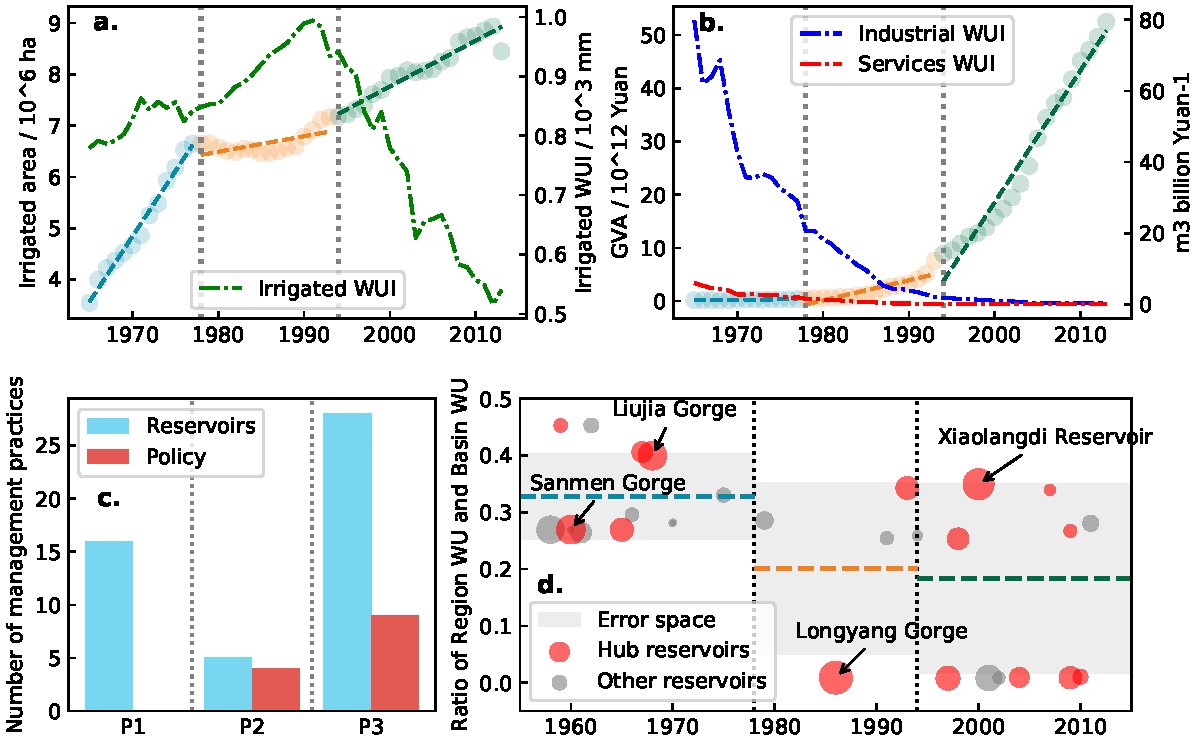
\includegraphics[width=\linewidth]{../../figures/main_text/causes.pdf}
	\caption{
		Causes of water utilization regime shifts: economy growths, efficiency changes, and managements.
		\textbf{A.} Changes of total irrigated area and water consumption per unit of irrigated area.
		\textbf{B.} Changes of gross values added (GVA) of industry and services, and their water use density (WUI) respectively (see supplementary: Methods. S2 for details).
		\textbf{C.} Constructions' finished time of each new reservoir and their located regions' water use percentages in basin's total water use, at that time. Red ones denote hub reservoirs in the basin, which plays a role in integrated water management. Size of the points indicates their magnitude of water storage capacities. Some important or special reservoirs' name are denoted: (1) Xiaolangdi reservoir and Sanmen Reservoir were constructed mainly responsible for managing sediments of the Yellow River. (2) Liujia Gorge, Longyang Gorge, were constructed mainly responsible for managing water flood discharge and storage. Therefore, these marked reservoirs are significant for the entire basin, far crucial than regional development.
	}
	\label{fig:Causes}
\end{figure}

Some main drivers caused the above changes of water utilization regime.
% 经济总量提升导致资源耗竭的加速。
(1) The expansion of irrigated area and the economic growth of industry and services are keys to the changes in the tendentiousness of water utilization between P1 and P2 (Figure\ref{fig:Causes} A). During the P1, irrigated agricultural area in the Yellow River basin expanded rapidly at a rate of $0.25*10^6/year$, and irrigation water was the dominant utilization way ($81.56\%$ of the total water use in 1965, and $83.17\%$ in 1978). Entering P2, however, while the expansion of irrigated area stalled, industry and services gradually took off and took up more water resources (Figure\ref{fig:Causes} B), leading to $8\%$ reduction of proportion of irrigation water.

% 用水关系的变化
(2) During the P3, irrigation, whose water consumptions were still dominating, have noticeable changes in its efficiency, however. Although irrigated agricultural area resumed expansion, and both industry, urban services were boosting their gross added values (GVA), water use density (WUI) experienced significant declines and reached the lowest points (Figure\ref{fig:Causes} A and B). It means, water utilization ways  have changed, along with technological solutions and a range of water conservation practices (supplementary Fig. S6). As a result, the proportions of water use between the different sectors tend to average out while the total water consumption remains stable, after the P3 (supplementary Fig. S7).

% 不断变化的管理模式。
(3) Changing water management practice contributed throughout all three periods. In the P1, most of the reservoirs are built in regions with high water demands, as ratio of regional water use and basinal water use for each new reservoir are significantly higher (Figure~\ref{fig:Causes}C). In the P2, on the other hand, the number of new reservoirs decreases significantly with little increment of total storage capacities (supplementary Fig. S5). Entering the P3, however, the number of new reservoirs are even much higher than that in the P1, and most of them were built in regions with lower ratio of regional water use and basinal water use (Figure~\ref{fig:Causes}C and supplementary Fig. S5).

% tag 讨论
\section*{Discussion}

\subsection*{Transition Framework}

\begin{figure*}[thbp]
	\centering
	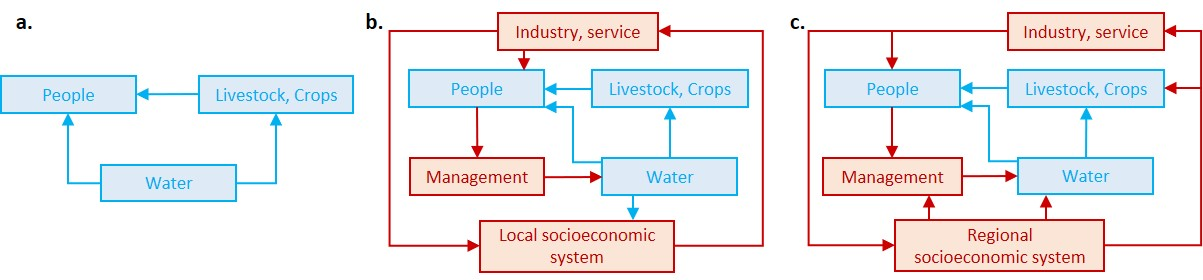
\includegraphics[width=\linewidth]{../../figures/main_text/framework}
	\caption{
		Transition framework of the water utilization regime towards natural-social binary cycle.
		\textbf{A. Natural cycle:} As a kind of direct provisioning resource, the main functions of water resource is to support crop, livestocks and human-beings, which are the basic ecological services.
		\textbf{B. Regional cycle:} With local socio-economic systems developing, industry and services (also known as the secondary and the tertiary industry) calling for further water consumptions.
		However, as their ecological services generated through the socio-economic cycle, water resources play a non-provisioning role. What's more, better organized socio-economic system and developed technology gives humans the will and ability to better manage water resources and change since this phase, with intensive intervention in the natural water cycle. 
		\textbf{C. Basinal cycle:} Entering this phase, with further developing in more economically efficient industries and services, trade-off between whose water demands with provisional water demands becomes prominent. Rather than determined by local socio-economic systems, water withdrawals and management act as considerations within the entire basin more, therefore. 
	}
	\label{fig:framework}
\end{figure*}

% 普遍存在的稳态转换可以由渐变或突变造成,而人类压力在世界范围内都是稳态转换最重要的驱动因素之一。
Widespread regime shifts in a human-water system can be triggered by accumulation of gradual changes, where increasing anthropogenic pressure are among the most important drivers \cite{rochaCascadingRegimeShifts2018a,falkenmarkUnderstandingWaterResilience2019}. 
% 而随着人类干预的加深,水循环出现了自然-社会二元结构,主导当前人水系统的互馈过程。
At the same time, human society has become more and more dependent on water utilization as it further develops, modifying natural water cycles by socio-economic processes \cite{gleesonIlluminatingWaterCycle2020,dibaldassarreSociohydrologyScientificChallenges2019}.
% 与社会-自然二元水循环理论
This social water cycle has linked to the natural water cycle through water withdraw, water utilization and drainage, forming a closed chain of interdependence, interconnection and mutual influence, which is consistent with nature-society dualistic water cycle theory 
\cite{qinTheoreticalFrameworkDualistic2014,liuDualisticWaterCycle2010}.
% 我们的研究结果表明,与社会-生态系统的过渡过程类似,水资源利用体系的变化也存在类似稳态转换的阶段性特征,并最终呈现出自然-社会二元结构。
According to our results, regime shifts of water utilization as transitional phases induced by developing, similar in social-ecological system, is one of the most important characteristics towards natural-social dualistic structure 
\cite{cummingImplicationsAgriculturalTransitions2014,cummingLinkingEconomicGrowth2018}.
% 因此,我们在总结黄河流域变化过程的基础上,进一步概念化了水资源利用制度的过渡框架。
As such, we summarized a transition framework of the water utilization regimes here, which conceptualizes a general trajectory towards a natural-social dualistic water cycle (Figure~\ref{fig:framework}).


% 水资源利用制度包括压力、倾向性、格局三个重要因素,三个指标在过渡框架中随着不断变化。
Throughout the above transition phases towards dualistic water cycle, three dimensions of water utilization regime are various in discipline of evolution, corresponding to typical changes within the Yellow River Basins as an example (Figure~\ref{fig:dimensions}). 
% 水资源压力
(1) Firstly, although stresses on water resources increases by economic expansion boosting water demands, socio-economic progress responding to resource scarcity by better management and efficiency. Water resources were becoming more scarce in the Yellow River Basin from P1 to P3, but the expansion of farmland, the construction of reservoirs, and the increase in water use efficiency became responses to different water utilization stresses in aspects (Figure~\ref{fig:Causes}). Since the scarcity of water resources is directly perceptible and sensitive for utilization, its stresses on societies is one of the most striking drivers to regime shifts within human-water systems \cite{qinFlexibilityIntensityGlobal2019}.
% 水资源倾向性
(2) Secondly, the non-provisioning part of water demands growths with secondary and tertiary industries developing, leading tendentiousness of water utilization continually tilted to the socio-economic part. As original region of Ancient Chinese Civilization, the Yellow River Basin used to be dominated by agricultural but in its way to an energy industry zone now \cite{WillEnergyBases}. As a result, saving water consumption in agriculture and making concessions for industry and energy is widely recognized as solutions for the competing \cite{xiangWillEnergyIndustry2016,bebbWaterRightsTransfers2011}. Anyhow, this changes of tendentiousness reflect a truth that growing socio-economic parts are throwing feedbacks to scarcity of water resources and contributing to regime shifts.
% 水资源格局
(3) Thirdly, with closer socio-economic ties and stiffer competition between regions and sectors, the geographic scope of water resource supply and demand allocation is expanding, leading to changing patterns of water utilization. In the Yellow River Basin, the gap in water consumptions between regions and sectors are narrowing, as the result of a carefully designed allocation \cite{wangThirtyYearsYellow2018}. However, the allocation of water utilization is determined on the basis of regional and sectoral economic contexts and development trajectories\cite{wangThirtyYearsYellow2018}. The changes in water utilization patterns along with regime shifts, therefore, are the outcomes of feedback loops within complex human-water systems.

% 综上所述
By combining the above three dimensions, water utilization regimes reflect a tendency of transitional evolution thoroughly. In addition to the Yellow River Basin, which is the focus of this study, human-water relations in major river basins around the world can be explained by the framework. For examples, Indus River, Mississippi River, and Danube River, whose water utilizations have all gone through a relatively natural phases, rapid developments and integrated management regimes. \cite{bestAnthropogenicStressesWorld2019,cummingResilienceBigRiver2011}. In summary, our proposed transitional framework for the nature-society dualistic water cycle is universal, for identify regime shifts of water utilization.

\subsection*{Development Traps}
% 不同的流域位于过渡的不同阶段,面临的问题也存在区别,主要包括资源陷阱和结构陷阱两类。
At different transition phases, basins may face to various development traps in water utilization, leading an unsustainable trajectory (Figure~\ref{fig:traps}). 
% 资源陷阱和失配,导致崩溃
Like social-ecological systems and other complex systems, coupled human-water system may collapse under the gradual pressure on resources or because of structural mismatches 
\cite{reyersSocialEcologicalSystemsInsights2018,cummingQuantifyingSocialEcologicalScale2020,wangCOSUSTMs0530Review}. 
% 转型应对陷阱
A number of studies have identified transformation as an important way out of unsustainable trajectory, and different types of transformation are required according to dominating phases and traps of systems \cite{scoonesTransformationsSustainabilityCombining2020a,steffenTrajectoriesEarthSystem2018}. 
% 我们的框架有助于理解和识别
Thus, our transition framework can identify regime shifts of water utilization, which can help to predict possible development traps.

\begin{figure}%[htbp]
	\centering
	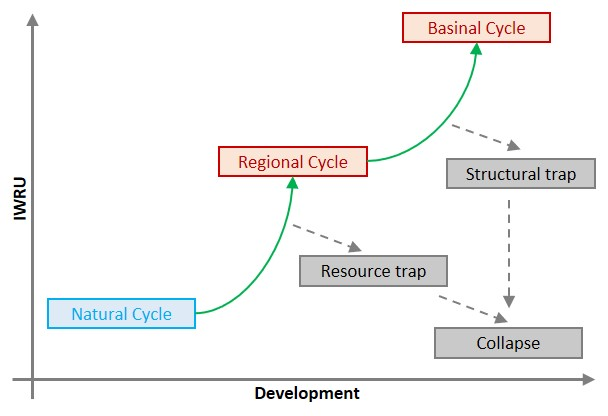
\includegraphics[width=\linewidth]{../../figures/main_text/traps.jpg}
	\caption{
		\textbf{Transition phases of water resources utilization regime and development traps.}
		Green arrows indicate the trajectory without falling into any development trap, IWRU roughly follows a non-linear upward trend at the same time. However, overexploitation of water resources will leave the system in a resource trap, without moving to regional coordinated cycle. And even if one enters a regional cycle, it can still fall into a structural trap when water utilization fails to adapt to the complex changes within human-water systems.
	}
	\label{fig:traps}
\end{figure}

% 世界各大流域面临的问题。资源开发早期容易陷入资源陷阱;流域发展后期容易陷入结构陷阱。
According to case studies around the world, big river basins often face resource traps at the beginning of their developments, while highly developed ones often face structural traps.
% 黄河流域的发展过程,资源开发P2阶段陷入了资源陷阱(表现形式 xxx)。
During P1 and P2 (refers from natural cycle to the regional cycle) in the Yellow River Basin, after the successive exploitation of agriculture, industry and services, the Water resource extraction rate has reached $79\%$, far exceeding the internationally recognized warning threshold of $40\%$. Although water management practices in P1 (construction of numerous reservoirs) mitigated the stress on water resources from accelerated development, it became scarce rapidly throughout and water utilization stresses rebounded in the P2 along with a regime shift. The resource trap is revealed at this point, with severe runoff outages and groundwater depletion of the Yellow River from P2 onwards (supplementary Fig. S8).
% 资源困局可能普遍存在
Since similar phenomena occurred in Mississippi and Indus River Basins, the fact that the accelerated development has been followed by water scarcity and a series of ecological problems shows that the resource traps is pervasive in the transition trajectory, especially from natural cycle to regional cycle 
\cite{bestAnthropogenicStressesWorld2019,cummingResilienceBigRiver2011}.

% 后来摆脱了资源陷阱(表现形式 xxx)。
To get rid of the resource trap, a clear transformation towards integrated basin management was proposed, with several management practices (supplementary Methods S4 and Fig. S9). The most important of these is the “87 Water Allocation Scheme”, which adopts a top-down approach in allocating water resources to all regions and sectors \cite{wangThirtyYearsYellow2018}. Since then, the scheme has been revised and refined, and a comprehensive water resources utilization system has gradually been formed that takes the basin scale into account \cite{wangThirtyYearsYellow2018}. These integrated management practices made the utilization of water resources into a regime of unified scheduling since the P3 in the Yellow River Basin, to escape from the “resource trap”. Similarly, many of the world's major river basins have eventually moved towards a system of integrated governance, especially for trans-boundary rivers (e.g. Danube and Mekong River), where water resources are in need of collaborative governance \cite{bodinCollaborativeEnvironmentalGovernance2017a}.


% 展望:未来还可能陷入结构陷阱,(表现形式:用水效率悖论的同时,倾向性停滞,灵活性进一步降低,)
However, in the regional cycle regime of water utilization, the Yellow River Basins still faces structural traps and require further transformation according to changes within the human-water system. 
Firstly, in line with paradox of irrigation efficiency, significant improvement in agricultural irrigation efficiency (i.e. decline in water use intensity) has been accompanied by a resurgence in irrigated area, resulting in an unabated and weak upward trend in water stress \cite{graftonParadoxIrrigationEfficiency2018}.
% 水资源压力仍在增大,而节水能力已经进入瓶颈,倾向性贡献减少)
Secondly, the changing tendentiousness between non-provisioning (i.e. industry and urban services) and provisioning (i.e. domestic and irrigation water use) is stagnating (see Figure~\ref{fig:dimensions}E) because of rigidify in the industrial structure. 
At the same time, the flexibility of water use is declining since domestic water use and thermal water use growth rapidly (supplementary Fig. S4). 
% 下一步:可以通过统一调控,调整格局来调整结构,突破结构陷阱。
% 总结:整个流域需进一步转型与适应,以实现高质量发展。
Typically, these may lead to a reduction in resilience of basins and leave highly coupled human-water systems facing greater vulnerability to collapse --as a structural trap \cite{cummingResilienceBigRiver2011}. Therefore, based on the identification of current phases and development traps by the transition framework, further transformative governance is still needed to achieve a high-quality sustainable development of the basin \cite{scoonesTransformationsSustainabilityCombining2020a}.




%tag 研究方法
\matmethods{
Here, we constructed the Integrated Water Resources Utilization (IWRU) Index which consists of three dimensions and identified the regime in the changes of the index over time by change points detection. Finally, the contribution to changes of IWRU index along with each main indicators were calculated separately for each regime (i.e. period). 
	
	\subsection*{Integrated Water Resources Utilization (IWRU) Index}
	The Integrated Water Resources Utilization (IWRU) Index consists of three dimensions (stresses, tendentiousnesses and patterns, denoted by sub-indicators correspondingly). Assuming they have equal weights, we log-transformed and standardized the three sub-indicators for elimination of differences between indicators. It means for each indicator $I_{sub}$, we performed:
	$$ I' = log(I_{sub}) $$
	$$ I = (I' - I'_{min}) / (I'_{max}-I'_{min})$$
	where $I$ is standardized series for $I_{sub}$.
	Then, since we assumed different relationships between development and sub-indicators, we added them together in equal weights:
	$$ IWRU = \sum_{i}^3 I'_i $$
	where $i$ is stress, tendentiousness or pattern, and $I'_i$ is standardized sub-indicator of them. A brief description of the sub-indicators used to measure each dimension follows (see SI Methods. S3 for more details).

	\subsubsection*{Sub-indicator of Stresses}
	Humans use technology to continuously manage water resources, so a simple physical water scarcity index cannot reasonably assess water scarcity in the evolution and transition of socio-water systems. Therefore, we refer to the scarcity-flexibility-variability (SFV) water stress index proposed in Qin et al., 2019 to evaluate water scarcity in the basin. The index takes into account management measures (such as the construction of reservoirs) and the impact of changes in the industrial structure of water use on the evaluation of water scarcity \cite{qinFlexibilityIntensityGlobal2019}.

	To apply this method, we need to combine three metrics following: 
	
	First for scarcity, $A_{i, j}$ is the total water consumption as a proportion of regional multi-year average runoff volume, in year $j$ and region $i$:
	$$ A_{i, j} = \frac{WU_{i,j}}{R_{i, avg}} $$
	Second for flexibility, $B_{i, j}$ is the inflexible water use $WU_{inflexible}$ (i.e. for thermal power plants or humans and livestock) as a proportion of average multi-year runoff, in year $i$ and region $j$:
	$$ B_{i, j} = \frac{WU_{inflexible}}{R_{i, avg}} $$
	Finally for variability, the capacity of the reservoir and the positive effects of storage on natural runoff fluctuations are also considered.
	$$ C_i = C1_i * (1 - C2_i) $$
	$$ C1_{i, j} = \frac{R_{i, std}}{R_{i, avg}} $$
	$$ C2_{i} = \frac{RC_{i}}{R_{i, avg}}, \ if RC < R_{i, avg} $$
	$$ C2_{i} = 1, \ if RC >= R_{i, avg} $$
	In all the equations above, $R_{i, avg}$ is the average runoff in region $i$, $RC_i$ is the total storage capacities of reservoirs in the region $i$, $R_{i, std}$ is the standard deviation of runoff in the region $i$.

	Finally, assuming three metrics (scarcity, flexibility and variability) have the same weights, we can calculate $SFV$ index after normalizing them:
	$$ V = \frac{A_{normalize} + B_{normalize} + C_{normalize}}{3} $$
	$$ a = \frac{1}{V_{max} - V_{min}}; $$
	$$ b = \frac{1}{V_{min} - V_{max}} * V_{min} $$
	$$ SFV = a * V + b $$

	\subsubsection*{Sub-indicator of Tendentiousness}
	To tendentiousness, we use non-provisioning shares of water use as an indicator. While provisional water use ($WU_{pro}$) includes domestic, irrigated and livestock water uses, the non-provisioning water use ($WU_{non-pro}$) includes industrial and urban services water uses. Then, we can calculate the non-provisioning shares by:
	$$ NPS_{ij} = \frac{WU_{indirect, i, j}}{WU_{direct, i, j} + WU_{undirect, i, j}} $$

	\subsubsection*{Sub-indicator of Patterns}
	To description of patterns between regions or sections, we designed an indicator by imitation of information entropy. Assuming the most egalitarian water allocation is assumed to be that each region or sectoral development utilizes the same proportion of water resources (the case of maximum entropy). The ratio between the actual water allocation entropy and this maximum entropy is the allocation entropy index.
	$$ ratio = \frac{Entropy}{Entropy_{max}} $$
	where $Entropy$ and $Entropy_{max}$ are entropy and maximum entropy of water distributions, respectively. They can be calculated by:
	$$ Entropy = \sum_{i=1}^n \sum_{j=1}^m -log(p_{ij}) * p_{ij} $$
	$$ Entropy_{max} = n * \sum_{j=1}^m -\frac{p_j}{n} * log(\frac{p_j}{n}) $$ 
	where $p_j$ and $p_ij$ are proportions of water use in sector $j$ and region $i$:
	$$ p_j = \frac{\sum_{i=1}^n WU_j}{\sum_{i=1}^n WU} $$
	$$ p_{ij} = \frac{WU_{ij}} {\sum_{i=1}^n \sum_{j=1}^m WU_{ij}} $$
	where $n$ is the total number of regions ($n=4$ here, see supplementary Methods. S1) and $m$ is the total number of sectors ($m=4$ here, see supplementary Methods. S2).

	\subsection*{Change points detection}
		The method makes no assumptions about the distribution of the data and detects breakpoints based solely on the probability of the data coming from different distributions before and after the breakpoint.
		The approach after Pettitt (1979) is commonly applied to detect a single change-point in hydrological series or climate series with continuous data \cite{pettittNonParametricApproachChangePoint1979}. It tests the $H0$: The variables follow one or more distributions that have the same location parameter (no change), against the alternative: a change point exists. The non-parametric statistic is defined as:
	
		$$ K_t = max|U_{t, T}|$$
		where:
		$$ U_{t, T} = \sum_{i=1}^t\sum_{j=t+1}^T sgn(X_i - X_j) $$
	
		The change-point of the series is located at $K_T$, provided that the statistic is significant. We use 0.001 as the threshold of p-value, which means the probability of a statistically significant change-point judgment being valid is more than $99.9\%$. Since this method only can return one significant change point, we repeat it Until all significant change points were detected.
	
	% 计算贡献度
	\subsection*{Contribution decomposition}
		We have decomposed the amount of variation in each index at different stages in order to observe the contribution of each influencing factor to them. Use Integrated Water Resources Utilization (IWRU) Index as an example, which influenced by three dimensions: stress ($S$), tendentiousness ($T$) and pattern ($P$) (indicated by their own index respectively, see Water utilization regime index and supplementary Methods. S3):
		$$ IWRU = T * P * S ^ {-1} $$
		Take the logarithm of both sides then, we get:
		$$ ln(IWRU) = ln(S) + ln(T) - ln(P) $$
		Since the changes of IWRU $\Delta IWRU$ can be expressed as $\Delta IWRU = ln(IWRU_2) - ln(IWRU_1)$, where $IWRU_2$ and $IWRU_1$ are ending and beginning values of IWRU in a certain time period, combining the above equations we can get:
		$$ \Delta IWRU = ln(\frac{S_1}{S_2}) + ln(\frac{T_2}{T_1}) + ln(\frac{P_2}{P_1}) = -\Delta S + \Delta T + \Delta P $$
		Then, we can calculate contributions $C_F$ of a certain factor $F$ in a certain period by:
		$$ C_{F} = \frac{|\Delta C_{F}|}{\Delta IWRU}$$
}

\showmatmethods{} % Display the Materials and Methods section

\acknow{Please include your acknowledgments here, set in a single paragraph. Please do not include any acknowledgments in the Supporting Information, or anywhere else in the manuscript.}

\showacknow{} % Display the acknowledgments section

% Bibliography
\bibliography{my-papers}
	
\end{document}